% Compile with XeLaTeX or LuaLaTeX
\documentclass[10pt,a4paper]{article}
\usepackage{xcolor}
\usepackage{titlesec}
\usepackage{fontspec}
\defaultfontfeatures{Mapping=tex-text}
\usepackage{xunicode}
\usepackage{xltxtra}
\usepackage{polyglossia}
\usepackage{indentfirst}             % 段首缩进

\setdefaultlanguage{english}
% 设置字体
\setsansfont{Calibri}
\setmainfont[BoldFont=SimHei]{STKaiti}
\usepackage{amsmath}
\usepackage{amsfonts}
\usepackage{amssymb}
\usepackage{graphicx}
% 设置页边距
%\usepackage[left=2cm,right=2cm,top=2cm,bottom=2cm]{geometry}
\usepackage{hyperref}

\usepackage{listings}
\definecolor{codegreen}{rgb}{0,0.6,0}
\definecolor{codegray}{rgb}{0.5,0.5,0.5}
\definecolor{codepurple}{rgb}{0.58,0,0.82}
\definecolor{backcolour}{rgb}{0.95,0.95,0.92}

\lstdefinestyle{mystyle}{
	backgroundcolor=\color{backcolour},   
	commentstyle=\color{codegreen},
	keywordstyle=\color{magenta},
	numberstyle=\tiny\color{codegray},
	stringstyle=\color{codepurple},
	basicstyle=\footnotesize,
	breakatwhitespace=false,         
	breaklines=true,                 
	captionpos=b,                    
	keepspaces=true,                 
	numbers=left,                    
	numbersep=5pt,                  
	showspaces=false,                
	showstringspaces=false,
	showtabs=false,                  
	tabsize=2
}

\lstset{style=mystyle}

% 新定义字体
\newfontfamily\song{SimSun}          % 宋体
\newfontfamily\hei{SimHei}           % 黑体
\XeTeXlinebreaklocale "zh"           % 中文断行

% Define light and dark Microsoft blue colours
\definecolor{MSBlue}{rgb}{.204,.353,.541}
\definecolor{MSLightBlue}{rgb}{.31,.506,.741}
% Define a new fontfamily for the subsubsection font
% Don't use \fontspec directly to change the font
\newfontfamily\subsubsectionfont[Color=MSLightBlue]{Times New Roman}
% Set formats for each heading level
\titleformat*{\section}{\Large\bfseries\sffamily\color{MSBlue}}
\titleformat*{\subsection}{\large\bfseries\sffamily\color{MSLightBlue}\song}
\titleformat*{\subsubsection}{\itshape\subsubsectionfont}

\author{张志勇\footnote{email: hh\_maizi@163.com}\\[2ex]
    北京小鸟看看科技有限公司\\[2ex]}
\title{mathmatical models from visual inertial slam}
\date{May 12, 2017}
\begin{document}

%%%% 段落首行缩进两个字 %%%%
\makeatletter
\let\@afterindentfalse\@afterindenttrue
\@afterindenttrue
\makeatother
\setlength{\parindent}{2em}  %中文缩进两个汉字位

\maketitle
%%%%%%%%%%%%%%%%%%%%%%%%%%%%%%%%%%%%%%%%%%%%%%%%%%%%%%%%%%%%%%%%%%%%%%%%%%%%
%% 目录
%%%%%%%%%%%%%%%%%%%%%%%%%%%%%%%%%%%%%%%%%%%%%%%%%%%%%%%%%%%%%%%%%%%%%%%%%%%%


%%%%%%%%%%%%%%%%%%%%%%%%%%%%%%%%%%%%%%%%%%%%%%%%%%%%%%%%%%%%%%%%%%%%%%%%%%%%
%% 摘要
%%%%%%%%%%%%%%%%%%%%%%%%%%%%%%%%%%%%%%%%%%%%%%%%%%%%%%%%%%%%%%%%%%%%%%%%%%%%
\section{abstract}


%%%%%%%%%%%%%%%%%%%%%%%%%%%%%%%%%%%%%%%%%%%%%%%%%%%%%%%%%%%%%%%%%%%%%%%%%%%%
%% 正文
%%%%%%%%%%%%%%%%%%%%%%%%%%%%%%%%%%%%%%%%%%%%%%%%%%%%%%%%%%%%%%%%%%%%%%%%%%%%

%%%%%%%%%%%%%%%%%%%%%%%%%%%%%%%%%%%%%%%%%%%%%%%%%%%%%%%%%%%%%%%%%%%%%%%%%%%%
%% 概述
%%%%%%%%%%%%%%%%%%%%%%%%%%%%%%%%%%%%%%%%%%%%%%%%%%%%%%%%%%%%%%%%%%%%%%%%%%%%

\section{short intro}
使用camera + IMU的方案来做SLAM/Odometry,一般被称作Visual-Inertial Odometry (VIO)或者Visual-Inertial Navigation System (VINS)。按照David Scaramuzza的分类方法,首先分成filter-based 和 optimization based 的两大类。进一步按照是否把图像特征信息加入状态向量来进行分类,可以分为loosely-couply 和tightly-coupled。几个经典的算法包括:
\paragraph{filter based}
\begin{description}
	\item[msckf] msckf没有作者本人的源代码,但是有别人的实现.
	\item[rovio] Robust Visual Inertial Odometry(有代码).
	\item[ssf and msf] Vision Based Navigation for Micro Helicopters (有代码).
\end{description}

\paragraph{optimization based}
\begin{description}
	\item[loosely coupled] "Inertial aided dense and semi-dense methods for robust direct visual odometry" 
	\item[tightly coupled okvis] "OKVIS: Open Keyframe-based Visual-Inertial SLAM."
	\item[tightly coupled orbslam] "Visual-Inertial Monocular SLAM with Map Reuse."
\end{description}

\subsection{main procedure}
流程与实现


%%%%%%%%%%%%%%%%%%%%%%%%%%%%%%%%%%%%%%%%%%%%%%%%%%%%%%%%%%%%%%%%%%%%%%%%%%%%
%% visual inertial slam 中的数学模型
%%%%%%%%%%%%%%%%%%%%%%%%%%%%%%%%%%%%%%%%%%%%%%%%%%%%%%%%%%%%%%%%%%%%%%%%%%%%
\subsection{Notations}
\subsection{Preliminaries}
\paragraph{Rieman manifold}

The skew symmetric matrices:
\begin{equation}
\mathbf{\omega}^\wedge =\begin{bmatrix}
\omega_1 \\
\omega_2 \\
\omega_3
\end{bmatrix}=\begin{bmatrix}
0, -\omega_3, \omega_2 \\
\omega_3, 0, -\omega_1 \\
-\omega_2, \omega_1, 0
\end{bmatrix}\qquad \in so(3)
\end{equation}

wedge operator converts an vector to its corresponding matrix, and the vee operator convert the skew symmetric matrix to an vector. if we have $S=\omega^{\wedge}$, then
\begin{equation}
S^{\vee}=\omega
\end{equation}

The exponential map(at identity): 指数映射是skew symmetric matrix 到 rotation matrix 的映射.
\begin{equation}
exp(\phi^\wedge)=I + \frac{\sin(\|\phi\|)}{\|\phi\|}\phi^\wedge + \frac{1-\cos(\|\phi\|)}{\|\phi\|^2} (\phi^\wedge)^2
\end{equation}

a first order exponential map:
\begin{equation}
exp(\phi^\wedge)\approx I + \phi^\wedge
\end{equation}

logarithm map at the identity:
\begin{equation}
\log(R)=\frac{\varphi \cdot (R-R^T)}{2\sin(\varphi)} \qquad 
with \varphi=\arccos(\frac{tr(R)-1}{2})
\end{equation}

the vectorized versions of the exponential and logarithm map: 向量与SO(3)的映射. 
\begin{subequations}
\begin{align}
Exp:  R^3 \rightarrow SO(3); \Phi \rightarrowtail exp(\Phi^{wedge}) \\
Log:  SO(3) \rightarrow R^3; R \rightarrowtail log(R)^{\vee}
\end{align}
\end{subequations}

Exp 的一阶估计:
\begin{equation}
Exp(\Phi + \delta \Phi)\approx Exp(\Phi)Exp(J_{r}(\Phi)\delta \Phi)
\end{equation}

Log 的一阶估计:
\begin{equation}
Log(Exp(\Phi)Exp(\delta \Phi))\approx \Phi + J_{r}^{-1}(\Phi)\delta \Phi
\end{equation}

another useful property of exponential map:
\begin{subequations}
	\begin{align}
	R Exp(\Phi) R^T &= exp(R \Phi ^{\wedge} R^T)=Exp(R\Phi)\\
	\Leftrightarrow Exp(\Phi) R &= R Exp(R^T \Phi)
	\end{align}
\end{subequations}

\paragraph{Uncertainty description in SO(3)}
\begin{equation}
\tilde{R} = R Exp(\epsilon), \quad \epsilon \thicksim \mathcal{N}(0, \Sigma)
\end{equation}

the cost function:
\begin{equation}
\mathcal{L}(R)=\frac{1}{2}||Log(R^{-1}\tilde{R})||_{\Sigma}^{2} + const = 
\frac{1}{2}||Log(\tilde{R}^{-1}) R||_{\Sigma}^{2} + const
\end{equation}
this is geodesic uncertainty $\Sigma^{-1}$.
\paragraph{Gauss-Newton on Manifold}
move this paragraph to the supplementes.

\subsection{MAP}
\paragraph{Notations}
\paragraph{model description}
the state:
\begin{equation}
x_{i} \doteq \begin{Bmatrix}
R_{i}, p_{i}, v_{i}, b_{i}
\end{Bmatrix}.
\end{equation}

Let $\mathcal{K}$ denote the set of all keyframes up to time \textit{k}, the state of all 
keyframes:
\begin{equation}
\mathcal{X}_k \doteq \{x_i\}_{i\in \mathcal{K}_k}
\end{equation}

the measurements:
\begin{equation}
\mathcal{Z}\doteq \{\mathcal{C}_i, \mathcal{I}_{ij}\}_{(i,j)\in \mathcal{K}_k}
\end{equation}

factor graphs and map estimation:
the psoterior probability of the variables $\mathcal{X}_k$ :
\begin{equation}
p(\mathcal{X}_k|\mathcal{Z}_k) \varpropto p(\mathcal{X}_0) p(\mathcal{Z}_k | \mathcal{X}_k)
=  p(\mathcal{X}_0) \prod_{(i,j)\in \mathcal{K}_k} p(\mathcal{C}_i, \mathcal{I}_{ij}|\mathcal{X}_k)
=  p(\mathcal{X}_0) \prod_{(i,j)\in \mathcal{K}_k} p(\mathcal{I}_{ij}|x_i, x_j) 
\prod_{i\in \mathcal{K}_k} \prod_{l \in \mathcal{C}_i} p(z_{il}|x_i)
\end{equation}

finally the map estimate:
\begin{equation}
\mathcal{X}_k^* \doteq {argmin}_{\mathcal{X}_k} -log_e p(\mathcal{X}_k|\mathcal{Z}_k)
\end{equation}
展开后得到,
\begin{equation}
argmin_{\mathcal{X}_k} ||r_0||_{\Sigma_0}^2 + \Sigma_{(i,j) \in \mathcal{K}_k}||r_{\mathcal{I}_{ij}}||_{\Sigma_{ij}}^2 + ||r_{\mathcal{C}_{il}}||_{\Sigma_\mathcal{C}}^2
\end{equation}



\subsection{IMU Model and Motion Integration}

\subsubsection{IMU Model}
\begin{equation}
	_{B}\tilde{\omega}_{WB}(t) = _{B}\omega_{WB}(t) + b^g(t) + \eta^g(t)
\end{equation}

\begin{equation}
_B\tilde{a}(t) = R^T_{WB}(t)(_Wa(t) - _wg) + b^a(t) + \eta^a(t)
\end{equation}

\subsubsection{Kinematic Model}
\begin{equation}
\dot{R_{WB}} = R_{WB}\quad {_B}\omega_{WB}^{\wedge}, \quad _W\dot{v} = _wa, \quad _w\dot{p}=_Wv,
\end{equation}

\paragraph{the discrete form}
assuming ${_W}a$ and $_B\omega_{WB}$ remains constant in the time interval ${[t, {t+\Delta t}]}$

\begin{equation}
R_{WB}(t+\Delta t) = R_{WB}(t) Exp(_B \omega_{WB} \Delta t)
\end{equation}

\begin{equation}
{_W}v(t+\Delta t) = {_W}v(t) + {_w}a(t)\Delta t
\end{equation}

\begin{equation}
{_W}p(t+\Delta t) = {_W}p(t) + {_W}v(t)\Delta t + \frac{1}{2} {_W}a(t) {\Delta t}^2
\end{equation}

all in all rewrite equations above, we get,

\begin{equation}
R(t+\Delta t) = R(t) Exp(( \tilde{\omega}(t) - b^g(t) - \eta^g(t)) \Delta t)
\end{equation}

\begin{equation}
v(t+\Delta t) =v(t) + g(t) \Delta t + R(t)(\tilde{a}(t) -b^a(t) - \eta^a(t)) \Delta t
\end{equation}

\begin{equation}
p(t+\Delta t) = p(t) + v(t)\Delta t + + \frac{1}{2}g\Delta t^2
 + \frac{1}{2} R(t)(\tilde{a}(t) -b^a(t) - \eta^a(t)) \Delta t^2
\end{equation}

\subsection{IMU pre-integration}

\paragraph{IMU integration for all $\Delta t$ between two consecutive frames at times i and j}
\begin{subequations}
\begin{align}
	R_j &= R_i \prod_{k=i}^{j-1} Exp((\tilde{\omega} - b^g_k - \eta^{gd}_k) \Delta t) \\
	v_j &= v_i + g\Delta_{ij} + \Sigma_{k=i}^{j-1} R_k(\tilde{a}_k - b_k^a - \eta_k^{ad}) \Delta t \\
	p_j &= p_i + \Sigma_{k=i}^{j-1}[v_k\Delta + \frac{1}{2}g \Delta t^2 +
	\frac{1}{2} R^k (\tilde{a}_k - b_k^a - \eta_k^{ad}) \Delta t^2]
\end{align}
\end{subequations}

\paragraph{relative motion increments}
\begin{subequations}
	\begin{align}
	\Delta R_{ij} & \doteq R_i^T R_j = \prod_{k=i}^{j-1} Exp((\tilde{\omega} - b^g_k - \eta^{gd}_k) \Delta t) \\
	\Delta v_{ij} &\doteq R_i^T(v_j - v_i -g \Delta t_{ij}) = \Sigma_{k=i}^{j-1} \Delta R_{ik}(\tilde{a}_k - b_k^a -\eta_k^{ad}) \Delta t\\
	\Delta p_{ij} &\doteq R_i^T (p_j - p_i - v_i\Delta t_{ij} - \frac{1}{2} \Sigma_{k=i}^{j-1}g\Delta t^2)= 
	\Sigma_{k=i}^{j-1}[\Delta v_{ik}\Delta t + \frac{1}{2}\Delta R_{ik}(\tilde{a}_k - b_k^a -\eta_k^{ad}) \Delta t^2]
	\end{align}
\end{subequations}

\subsubsection{Preintegrated IMU Measurements}
\begin{subequations}
	\begin{align}
	\Delta R_{ij} &\simeq \prod_{k=i}^{j-1}[Exp((\tilde{\omega}_k - b_i^g) \Delta t) 
	Exp(-J_r^k \eta_k^{gd}\Delta t)]\\
	&= \Delta \tilde{R}_{ij} \prod_{k=i}^{j-1}Exp(-\Delta \tilde{R}_{k+1j}^{T} J_r^k \eta_k^{gd} \Delta t)\\
	&\doteq \Delta \tilde{R}_{ij} Exp(-\Delta \phi_{ij})
	\end{align}
\end{subequations}
... 类似可得到 $\Delta v_{ij}$ 和 $\Delta p_{ij}$.\\
接下来就是 “preintegrated measurement model”。
\begin{subequations}
	\begin{align}
		\Delta \tilde{R}_{ij} &= R_i^T R_j Exp(\delta \phi_{ij}) \\
		\Delta \tilde{v}_{ij} &= R_i^T(v_j - v_i -g \Delta t_{ij}) + \delta v_{ij}\\
		\Delta p_{ij}         &= R_i^T (p_j - p_i - v_i\Delta t_{ij} - \frac{1}{2} g\Delta t_{ij}^2) + \delta p_{ij}
	\end{align}
\end{subequations}

\subsubsection{Noise Propagation}
最终可以证明$\phi_{ij})$, $\delta v_{ij}$ 和 $\delta p_{ij}$ 是 $\eta_k^{gd}$ 的线性函数,服从高斯分布。

\subsubsection{Incorporating Bias Updates, given a bias update: $b \leftarrow \bar{b} + \delta b$}
\begin{subequations}
	\begin{align}
	\Delta \tilde{R}_{ij}(b_i^g)  &\simeq \Delta \tilde{R}_{ij}(\bar{b}^g) 
	Exp(\frac{\partial \Delta \bar{R}_{ij}}{\partial b^g} \delta b_i^g)\\
	\Delta \tilde{v}_{ij}(b_i^g, b_i^a) &\simeq \Delta \tilde{v}_{ij}(\bar{b}_i^g, \bar{b}_i^a) + 
	\frac{\partial \Delta \bar{v}_{ij}}{\partial b^g} \delta b_i^g + 
	\frac{\partial \Delta \bar{v}_{ij}}{\partial b^a} \delta b_i^a\\
	 \Delta \tilde{p}_{ij}(b_i^g, b_i^a) &\simeq \Delta \tilde{p}_{ij}(\bar{b}_i^g, \bar{b}_i^a) +
	 	\frac{\partial \Delta \bar{p}_{ij}}{\partial b_i^g} \delta b_i^g + 
	 \frac{\partial \Delta \bar{p}_{ij}}{\partial b^a} \delta b_i^a\\
	\end{align}	
\end{subequations}

\subsubsection{Bias Model}
Bias are slowly time-varying quantities, Hence model them with a "Browian Motion".
For more info, see \href{http://www.cnblogs.com/youzx/p/6291327.html?utm_source=itdadao&utm_medium=referral}{IMU Model}
\begin{equation}
\dot{b}^g(t) = \eta^{bg}, \quad \dot{b}^a(t) = \eta{ba}
\end{equation}

the discrete form.
\begin{equation}
b^g_j= b^g_i + \eta^{bgd}, \quad b^a_j= b^a_i + \eta^{bad},
\end{equation}

covariance of discrete bias.
\begin{equation}
\Sigma^{bgd} \doteq \Delta t_{ij} Cov(\eta^{bg}), \quad \Sigma^{bad} \doteq \Delta t_{ij} Cov(\eta^{ba}),
\end{equation}

factor graph of bias model.
\begin{equation}
||r_{b_{ij}} ||^2 \doteq ||b_j^g - b_i^g||_{\Sigma^{bgd}}^2 + ||b_j^a - b_i^a||_{\Sigma^{bad}}^2
\end{equation}

\subsection{Linearizing expression for nonlinear optimization}
\paragraph{linearizing rotation matrix}
\paragraph{transformation matrix}
\paragraph{linearizing homogeneous points}
\paragraph{examples on stereo camera}
\subsection{}
\subsection{}
\subsection{}
\subsection{}

\section{mathematical principles behind the model}
\subsubsection{Preliminaries}
\subsubsection{Notions of Riemannian geometry}
\subsubsection{Uncertainty descriptions in SO(3)}
\subsubsection{Gauss-Newton Method on Manifold}

\subsection{Maximum a Posteriori visual-inertial state estimation}

\section{Problems still working on}
\begin{itemize}
	\item right jacobian and left jacobian
	\item 
\end{itemize}

%%%%%%%%%%%%%%%%%%%%%%%%%%%%%%%%%%%%%%%%%%%%%%%%%%%%%%%%%%%%%%%%%%%%%%%%%%%%
%% 流程与实现
%%%%%%%%%%%%%%%%%%%%%%%%%%%%%%%%%%%%%%%%%%%%%%%%%%%%%%%%%%%%%%%%%%%%%%%%%%%%


%%%%%%%%%%%%%%%%%%%%%%%%%%%%%%%%%%%%%%%%%%%%%%%%%%%%%%%%%%%%%%%%%%%%%%%%%%%%
%% 补充材料
%%%%%%%%%%%%%%%%%%%%%%%%%%%%%%%%%%%%%%%%%%%%%%%%%%%%%%%%%%%%%%%%%%%%%%%%%%%%
\section{supplementaries}
\subsection{高斯噪声与随机游走}
\subsection{IMU的工作原理与机制}
\subsection{gtsam 与isam}
\subsection{matrix calculus}

%%%%%%%%%%%%%%%%%%%%%%%%%%%%%%%%%%%%%%%%%%%%%%%%%%%%%%%%%%%%%%%%%%%%%%%%%%%%
%% 参考文献
%%%%%%%%%%%%%%%%%%%%%%%%%%%%%%%%%%%%%%%%%%%%%%%%%%%%%%%%%%%%%%%%%%%%%%%%%%%%

%%%%%%%%%%%%%%%%%%%%%%%%%%%%%%%%%%%%%%%%%%%%%%%%%%%%%%%%%%%%%%%%%%%%%%%%%%%%
%\subsubsection{}
%演示代码插入效果:
%\begin{lstlisting}[title=sd\_method.m, frame=shadowbox]
%point = [9; 1];
%H = [1, 0; 0, 9];
%figure
%ezcontour('x^2/2+9*y^2/2',[-9, 9, -6, 6])
%
%% steptest decent method
%sdm_points = [9; 1];
%count = 0;
%while(norm(point) > 1e-5)
%    count = count + 1;
%    g = [point(1); 9*point(2)];
%    point = point - g'*g/(g'*H*g).*g;
%    sdm_points = [sdm_points, point];
%end
%hold on
%plot(sdm_points(1, :), sdm_points(2, :),'-','LineWidth',3);
%count
%\end{lstlisting}
%图片插入效果图:
%    \begin{center}
%		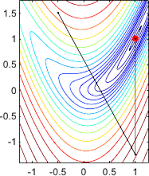
\includegraphics[width=1\textwidth]{images/GN.png}
%	\end{center}
\end{document}